\documentclass[12pt]{article}
\usepackage{fancyhdr} % for custom headers and footers
\usepackage[utf8]{inputenc} % support for UTF-8 encoding
\usepackage{geometry} % for page layout
\geometry{a4paper, margin=1in} % set A4 paper and margin
\usepackage{lipsum}  % For generating dummy text
\usepackage[T1]{fontenc}
\usepackage{newpxtext,newpxmath}  % Using Palatino font
\usepackage{hyperref}
\usepackage{pdfpages}
% \usepackage{lmodern}
% \usepackage{helvet}

\setcounter{secnumdepth}{2}
% 设置文献样式为 IEEE
\usepackage[style=ieee]{biblatex}


\setlength{\headheight}{15pt}

\addbibresource{references/reference.bib}  % 指定文献数据库


% 定义课程名称宏
\newcommand{\coursename}{DAT094}
\newcommand{\labname}{What constitutes a good lab report?}

% Define a custom command for inserting images
% Arguments:
% 1: Filename
% 2: Width (as a fraction of \textwidth)
% 3: Caption
% 4: Label

\newcommand{\insertimage}[4]{
    \begin{figure}[htbp]
        \centering
        \includegraphics[width=#2\textwidth]{#1}
        \caption{#3}
        \label{#4}
    \end{figure}
}


% - This file defined the format of code blocks.

\usepackage{listings} % For syntax highlighting
\usepackage{xcolor} % For defining custom colors

% Define custom colors
\definecolor{commentgreen}{rgb}{0.25,0.5,0.35}
\definecolor{keywordblue}{rgb}{0,0.2,0.6}
\definecolor{backcolour}{rgb}{0.95,0.95,0.92}

% Define the language style for QuestaSim .do files
\lstdefinelanguage{questasim}{
  morekeywords={vlog, vsim, add, wave, do, run, quit, onbreak, resume, stop, set, show}, % Add other keywords as necessary
  morecomment=[l]{//}, % Line comment style
  morestring=[b]", % String style
  sensitive=false, % Keywords are not case-sensitive
  morestring=[b]' % Single quote strings
}

% Set the overall listing style
\lstset{
  language=questasim,
  backgroundcolor=\color{backcolour},
  commentstyle=\color{commentgreen},
  keywordstyle=\color{keywordblue}\bfseries,
  stringstyle=\color{red},
  basicstyle=\ttfamily,
  breakatwhitespace=false,   
  breaklines=true,           
  captionpos=b,            
  keepspaces=true,           
  numbers=left,              
  numbersep=5pt,             
  showspaces=false,          
  showstringspaces=false,
  showtabs=false,             
  tabsize=2,
  frame=single
}



\lstset{
    language=[LaTeX]TeX, % 设定为LaTeX语言
    basicstyle=\ttfamily, % 使用等宽字体
    keywordstyle=\color{blue}, % 关键字使用蓝色
    commentstyle=\color{commentgreen}, % 注释使用绿色
    stringstyle=\color{red}, % 字符串使用红色
    breaklines=true, % 自动换行
}


% - This file defined the format of question blocks.

% 加载 tcolorbox 和 xcolor 包
\usepackage{tcolorbox}
\usepackage{xcolor}

% 定义一个定制的 tcolorbox 环境
\newtcolorbox[auto counter]{questionbox}[1][]{%
    colback=red!10!white,
    colframe=red!55!black,
    title=Question \thetcbcounter,
    #1
}



\usepackage{titlesec} % For section title customization

% Optional: Customize the font
% \usepackage[T1]{fontenc}
% \usepackage{lmodern} % Using a slightly nicer font

% Enhance title format
\newcommand{\hsp}{\hspace{20pt}}
\titleformat{\section}[block]{\large\bfseries\filcenter}{}{1em}{}



% Custom title layout
\title{
    \vspace{-2.5cm} % Reduce the vertical space above the title
    \textbf{\Large \coursename} \\[5pt] % Reduce space before the rule
    \textbf{\Large \labname} \\[-10pt] % Reduced vertical spacing
    \rule{\textwidth}{1pt} \\[-10pt] % Horizontal rule with negative space to pull text up
    \begin{tabular}{@{}p{\textwidth}@{}} % Full width tabular
        \small \textbf{Chen Wu} \hfill  \small \textbf{\today}
    \end{tabular}
}
\date{} % Remove the default date display
\author{} % Clear the author to manage it manually in the title

% Enhance title format with numbering
\titleformat{\section}
  {\large\bfseries\filcenter}  % format
  {\thesection.}               % label (section number)
  {1em}                        % sep (space between number and title text)
  {}                           % before-code
  


\begin{document}

\maketitle
\pagestyle{fancy}
\fancyfoot[C]{\thepage} % center page number in the footer
\fancyhead[L]{\labname} % "Experiment Report" on the left header
\fancyhead[R]{\coursename} % course name on the right header

% ---Abstract---
\section*{Abstract}

Over the past few years, I have completed numerous experiment reports for various courses. 
As time has progressed, a relatively clear understanding of what constitutes an effective laboratory report has developed in my mind.
At the same time, with the help of writing guide from Chalmers\cite{ChalmersGuide}, deeper cognition on it generated in my mind.
Next, I will discuss this topic from three aspects: pre-writing consideration, structure and format, and specific implementation. 
In the first aspect, having a concept of writing purposes and audience is the most important. 
Secondly, from a formal perspective, a relatively fixed structure and format have more advantages. 
Besides, we finally discuss how to \("\)implement\("\) a report writing, including several methods to make a report more formal, aesthetic, and effective.

% ---Pre-writing---
\section{Pre-writing Consideration}

What constitutes a wonderful report?
Is that can only talk about the specific content in the report itself?
Actually, author's prior thinking is also an important part because it will instruct their subsequent writing.
From the website of Chalmers writing guide, several crucial questions which author should pay attention to have been mentioned, of which the most important two are purpose and audiences.

With the guide from the school's official website\cite{ChalmersGuide_pre-writing}, in pre-writing phase, determining who are audience is the first and foremost question.
Thus, before we're talking about the specific structure and content in a report article, the first task is to ascertain audience.
Then, we can infer their potential purposes so that what should author mention and which part of our article should be emphasised will be confirmed.

Without any doubt, the task publishers and reviewers, our professor and teacher assistants are guaranteed ones.
For them, generally have three points to focus: whether students have done their mandatory tasks, checking the answers given by students to the question mentioned in task sheets, evaluating their understanding level. 
In the following, I will discuss how to perform better in a report for each point.

For the first one, students should follow the guide of task book carefully, and give powerful evidence to demonstrate you accomplished all steps and design, ranging from screenshots to well-designed code snippets.
Secondly, there are questions related to key concepts you should know in a lab manual generally, and are delving into it when you're completing is the best method.
Simultaneously, we also need to develop an in-depth understanding before we're writing the answers and reflect on it.
Besides, from the perspective of professor, show your accomplishment and answers more noticeable by utilizing several measures are preferred because such a strategy will make their work more effective.
We will give some specific method to realize it in the following sections, however, is the professor the only reader?

Lab reports are also meaningful for the students.
First and foremost, a report can serve as part of students' note system, the so-called second brain, which can always help remind you of important things.
Generally, a good report records what I did and what happened when you try to complete your lab task, and, obviously, with the appropriate coursework design, such recording will likely can as a reference when a student starts a new project or faces some similar challenges you had met in your future career.
So, when writing a report, especially a good and meaningful one, thinking about how it will contribute to you in the future is significant in pre-planning.

Secondly, writing a report thoughtfully and diligently will contribute to our skill improvement.
As mentioned above, a good report contains author's well-developed comprehension of knowledge, and however, writing itself usually servers as a catalyst for elevating your grasp.
When you put your thinking down to the \("\)paper\("\), you must consider it more comprehensively and carefully.
Apart from the parts related to the experiment itself, writing skills will also be improved when you're preparing a good lab report.
This is a wide concept that consists of various aspects of writing skills, including the use of academic language and structure, and also the application of technical tools, such as \LaTeX.

% ---Structure and Format---
\section{Structure and Format}

After building a comprehensive pre-writing consideration, how to design an appropriate article structure and format becomes the next question needs to be addressed.
In other words, what is the structure and format for a good experiment report?

Firstly, traditional logical flow structure is necessary, but it needs to be refined and modified.
The traditional structure likes an official journal paper, following the sections: abstract, introduction, methodology, results, and discussion.
Generally, it appears in any scientific journal because it gives a distinct path for other researchers to explain how they realize it and how others can reproduce it.
In a lab exercise designed by a professor, actually, the path is relatively fixed, and it is also not the important part compared to your personal suggestion and optimization.
Although it seems that directly showing your answers and experimental results is the most efficient way to prove your workload to the teacher, this pattern will deprive the chance of improving writing skills and make it a wired article rather than a completed report.
However, the detailed information can be found in guide manuals, so the \("\)introduction\("\) should serve as an excerpt of the key content in guidance, and \("\)methodology\("\) can be simplified unless it involves your personal designs rather than a repetition of guidelines.
In summary, the template structure finally is proposed: abstract, introduction, experiment process, results and discussion, appendix and references.


The structure of the provided template document is as follows:

\begin{enumerate}
    \item Abstract: \\A brief overview of the experiment report, summarizing its objectives and findings.
    \item Introduction: \\Provides background and details on the purpose of the experiment.
    \item Experiment Process: \\Describes the specific steps and procedures carried out during the experiment.
    \item Results and Discussion: \\Presents the results obtained from the experiment and discusses their significance.
    \item Appendix: Challenges and Solutions: \\An appendix that details any challenges faced during the experiment and the solutions implemented.
\end{enumerate}

The above structure is designed based on what is a good report in my mind.
In addition, apart from consider the main structure, maintaining a unified format or visual style is also important because it will enhance the readability of your reports and make it more aesthetic.
Nowadays, to create a \LaTeX \ template and customize it for every single class and laboratory task on online \LaTeX \ compiling platform overleaf is an advisable workflow.
I created a template and set some convenient interface for quickly changing the title and course name for improving portability.
Author can define some specific display approaches in person, such as the following blocks:


\begin{questionbox}
This is an example of question in lab assignment.
\end{questionbox}

\begin{lstlisting}[caption={Example QuestaSim .do File}, label={lst:questasim_example}, language=questasim]
// This is an example code block.
vlog my_module.v
vsim my_module
add wave -position end sim:/my_module/*
run -all
quit
\end{lstlisting}

It is also a noticeable way to emphasize personal answers and designs here.
Students can use the vivid color to guide reviewers to directly to find the part they should pay attention to.

% ---Specific Implementation---
\section{Implementation Details}

For now, we have discussed what a good report looks like, the content and framework of it.
There is also something behind a smart report which I think it is necessary for writing a report effectively and beneficially for a student.
Specifically, some effective implementation details are both useful for just writing a lab report and for further personal career.

Then, I will give some simple but meaningful advice just based on my experience.
Firstly, in \LaTeX , when we try to construct a block I mentioned before is quite wordy, and so, we can new a command (like Macros in programing languages):

\begin{lstlisting}[language=LaTeX,label={lst:LaTeX_block}]
% If we use \newcolorbox to create a category "question_box" rather than copy it every time
\newtcolorbox[auto counter]{question_box}[1][]{%
    colback=red!10!white,
    colframe=red!55!black,
    title=Question \thetcbcounter,
    #1
}

% An example
\begin{question_box}
This is an example of question in lab assignment.
\end{question_box}

\end{lstlisting}

Secondly, users can also use \("\)input\("\) command to simplify the main source file and make writers focus on the main body of an article easily.
In this template, I set some external files to greatly shorten the line counts of the main file.

\begin{lstlisting}[language=LaTeX]
% - This file defined the format of code blocks.

\usepackage{listings} % For syntax highlighting
\usepackage{xcolor} % For defining custom colors

% Define custom colors
\definecolor{commentgreen}{rgb}{0.25,0.5,0.35}
\definecolor{keywordblue}{rgb}{0,0.2,0.6}
\definecolor{backcolour}{rgb}{0.95,0.95,0.92}

% Define the language style for QuestaSim .do files
\lstdefinelanguage{questasim}{
  morekeywords={vlog, vsim, add, wave, do, run, quit, onbreak, resume, stop, set, show}, % Add other keywords as necessary
  morecomment=[l]{//}, % Line comment style
  morestring=[b]", % String style
  sensitive=false, % Keywords are not case-sensitive
  morestring=[b]' % Single quote strings
}

% Set the overall listing style
\lstset{
  language=questasim,
  backgroundcolor=\color{backcolour},
  commentstyle=\color{commentgreen},
  keywordstyle=\color{keywordblue}\bfseries,
  stringstyle=\color{red},
  basicstyle=\ttfamily,
  breakatwhitespace=false,   
  breaklines=true,           
  captionpos=b,            
  keepspaces=true,           
  numbers=left,              
  numbersep=5pt,             
  showspaces=false,          
  showstringspaces=false,
  showtabs=false,             
  tabsize=2,
  frame=single
}



\lstset{
    language=[LaTeX]TeX, % 设定为LaTeX语言
    basicstyle=\ttfamily, % 使用等宽字体
    keywordstyle=\color{blue}, % 关键字使用蓝色
    commentstyle=\color{commentgreen}, % 注释使用绿色
    stringstyle=\color{red}, % 字符串使用红色
    breaklines=true, % 自动换行
}


% - This file defined the format of question blocks.

% 加载 tcolorbox 和 xcolor 包
\usepackage{tcolorbox}
\usepackage{xcolor}

% 定义一个定制的 tcolorbox 环境
\newtcolorbox[auto counter]{questionbox}[1][]{%
    colback=red!10!white,
    colframe=red!55!black,
    title=Question \thetcbcounter,
    #1
}



\usepackage{titlesec} % For section title customization

% Optional: Customize the font
% \usepackage[T1]{fontenc}
% \usepackage{lmodern} % Using a slightly nicer font

% Enhance title format
\newcommand{\hsp}{\hspace{20pt}}
\titleformat{\section}[block]{\large\bfseries\filcenter}{}{1em}{}



% Custom title layout
\title{
    \vspace{-2.5cm} % Reduce the vertical space above the title
    \textbf{\Large \coursename} \\[5pt] % Reduce space before the rule
    \textbf{\Large \labname} \\[-10pt] % Reduced vertical spacing
    \rule{\textwidth}{1pt} \\[-10pt] % Horizontal rule with negative space to pull text up
    \begin{tabular}{@{}p{\textwidth}@{}} % Full width tabular
        \small \textbf{Chen Wu} \hfill  \small \textbf{\today}
    \end{tabular}
}
\date{} % Remove the default date display
\author{} % Clear the author to manage it manually in the title

% Enhance title format with numbering
\titleformat{\section}
  {\large\bfseries\filcenter}  % format
  {\thesection.}               % label (section number)
  {1em}                        % sep (space between number and title text)
  {}                           % before-code
  
\end{lstlisting}



\section*{Appendix}

Comment:

For the article:
although I try to write it more officially and academically, there are so many inappropriate expressions.
To be honest, I am not an experienced writer in academic writing, so I often struggle with structuring my ideas clearly and using the appropriate language.
However, I am committed to improving and learning through practice in future lab reports.

For the template:
it is a little complex in some situations, I do not think it is suited for every student.
I also do not think a compulsory template is a good choice in a course.
However, a series of well-designed templates, designed for different students respectively, could save everyone's time and energy.

The  \LaTeX  template file can be found here on overleaf website: \\
\url{https://cn.overleaf.com/read/tknbnrtfyvvd#b4da39}

It can also be found at GitHub:\\
\url{https://github.com/wenruoxu/lab-report-template}

Here is an example PDF file generated by such a template file:

%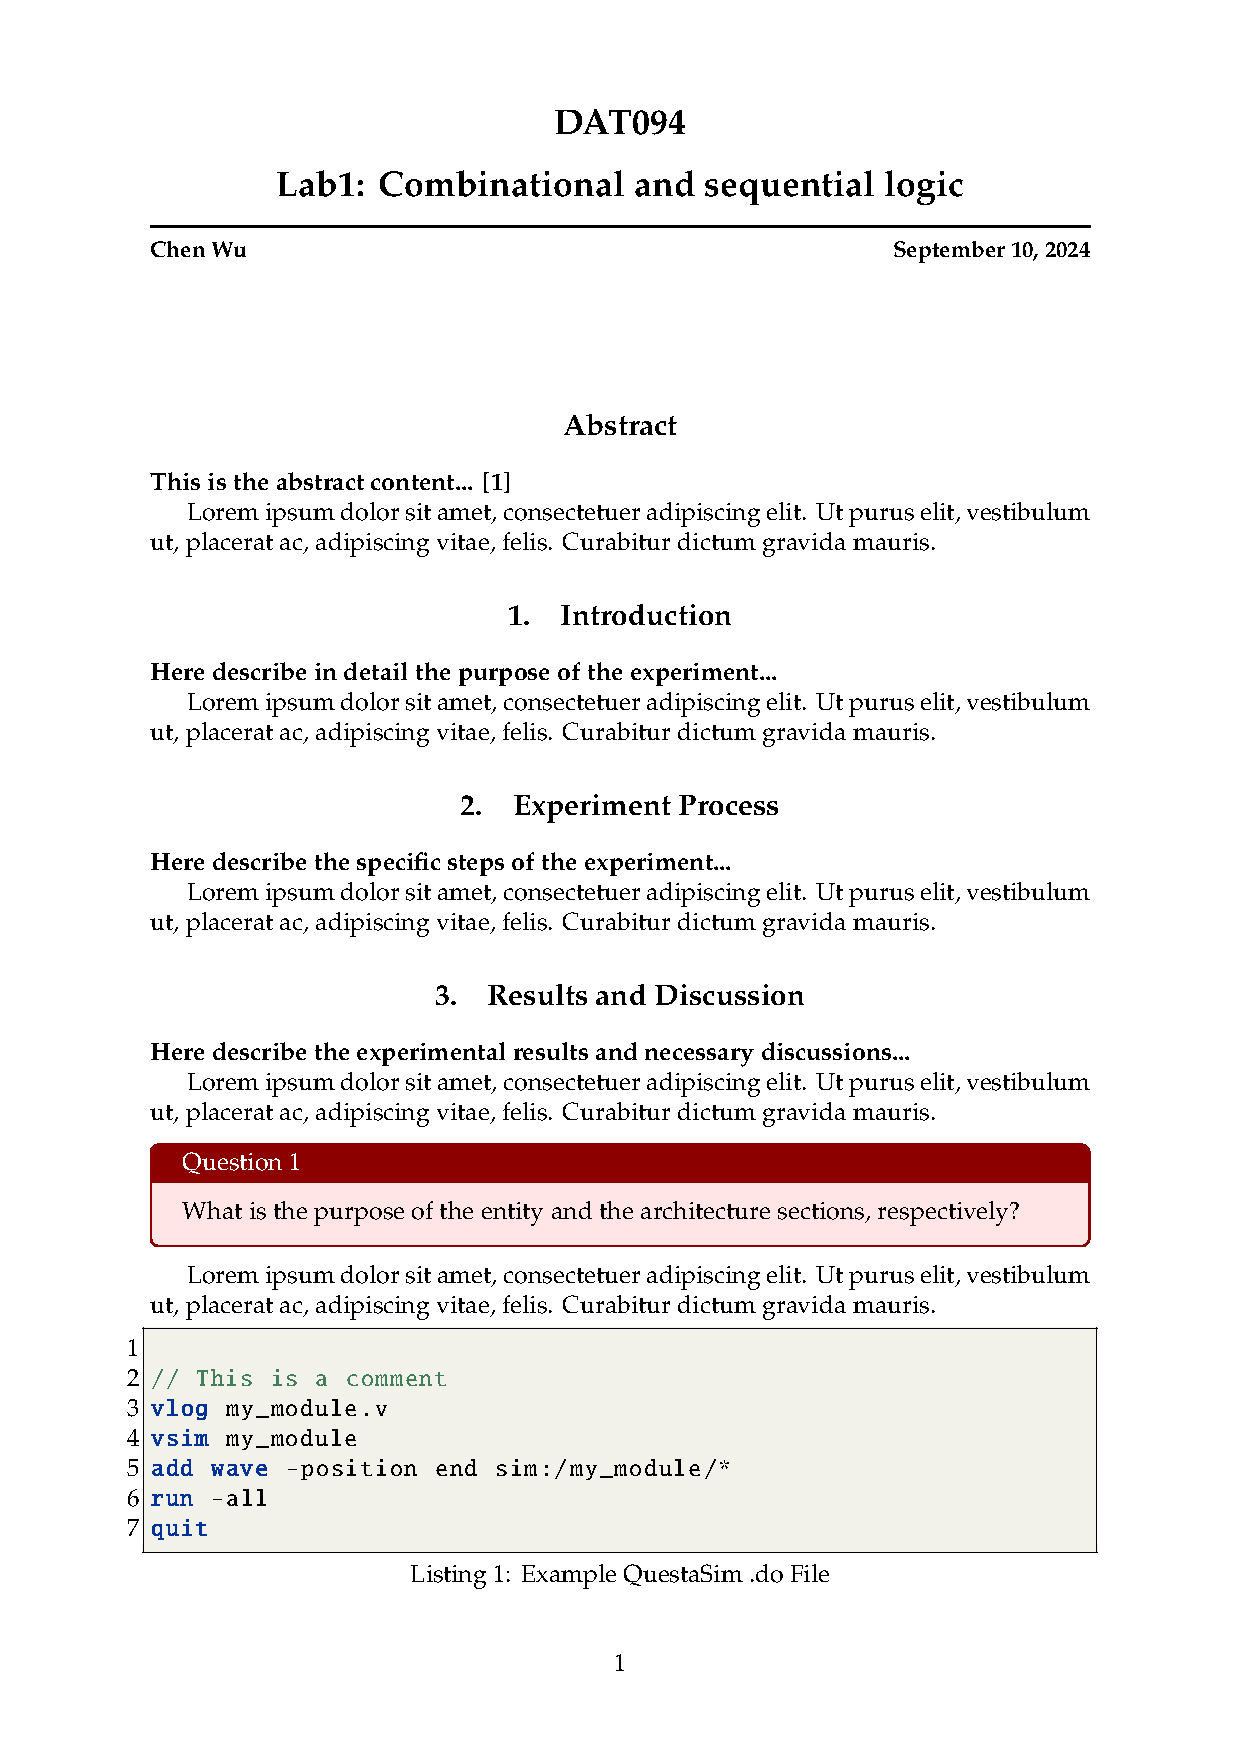
\includepdf[pages=-]{template_cutted.pdf} % 将example.pdf替换为你的PDF文件名

\newpage

\printbibliography

\end{document}
